Fairness entails more than the question whether are lottery numbers from the expected distribution. We need to search for deeper patterns in the data.
Thus a more comprehensive test is required to establish a more detailed answer to our question. We reformulate winning numbers
of a lottery as a stream of (supposedly) random bits. This enables us to deploy standard statistical suites for testing pseudo random number
generators.

Donald Knuth presented an initial set of empirical tests in the second volume of his computer science bible The Art of Computer Programming in 1969.
Since then numerous new test suites have been developed~\cite{HAC,NISTBible,dieharder,testu01}. We decided to use George Marsaglia's
Diehard battery of tests~\cite{diehard}. Diehard has been superceded by newer tests for its original purpose~\cite{dieharder}, however
it remains the best choice for us because it requires the least amount of data to run as illustrated in Figure \ref{fig:requirements}
and~\cite{datasize-dieharder}. Nonetheless even less data greedy test still requires quite a lot of data.
We are thus limited in which tests we can run given our dataset size.
\begin{figure}
    \centering
    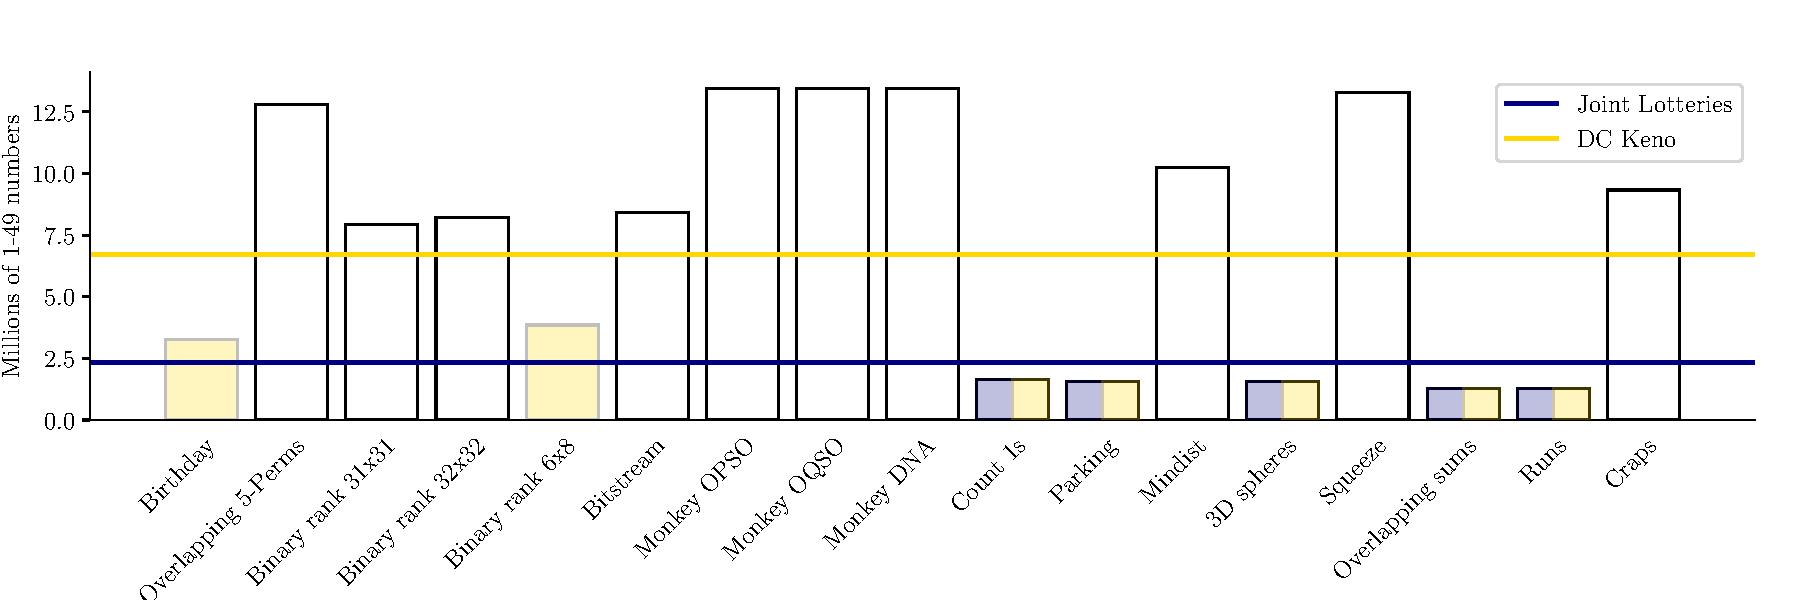
\includegraphics[width=\textwidth]{diehard_requirements.pdf}
    \caption{Amount of data required to run tests at default settings.}
    \label{fig:requirements}
\end{figure}
\todo{Transform figure into number of standard draws 1-49}

\subsection{Data augmentation}

Diehard battery expects a random stream of zero and one bits as input. We therefore require a function which produces uniformly
distributed bit sequences from lottery numbers. Because it is impossible to directly transform a discrete $\mathcal{U}(1, 49)$
of lottery numbers into $\mathcal{U}(0, 31)$ (the uniform distribution for 5-tuples of bits) we simply reject all numbers greater
than 32 and substract one from the rest. This causes a fair amount of data loss, but we do not see a better way.
(If a lottery draws from interval e.g. 1-80, we can throw away everything greater than 64 and get uniform distribution of bit 6-tuples.)

\subsection{Results}

The Diehard battery of tests provides 15 statistical tests. These tests operate with the null hypothesis that the data is truly random.
Each of them outputs one or more p-values, which are uniformly distributed if the null hypothesis is correct~\cite{NISTBible}.
In some cases, a Kolmogorov-Smirnov test is used to test for uniformity of p-values provide a single final, composite p-value. For more
information on the nature of these tests, consult either the Diehard source code appended to this report or one of George Marsaglia various
papers~\cite{monkey,mindist}.

We compare our lottery datasets against randomness collected from /dev/urandom, the preferred source of randomness in Linux
systems~\cite{manrandom,mythsrandom}. These datasets ensure that tests are working as intended and represent the best digital randomness
available to the common man.

\begin{figure}
    \centering
    \captionsetup[subfigure]{justification=centering}
    \begin{subfigure}{0.495\textwidth}
        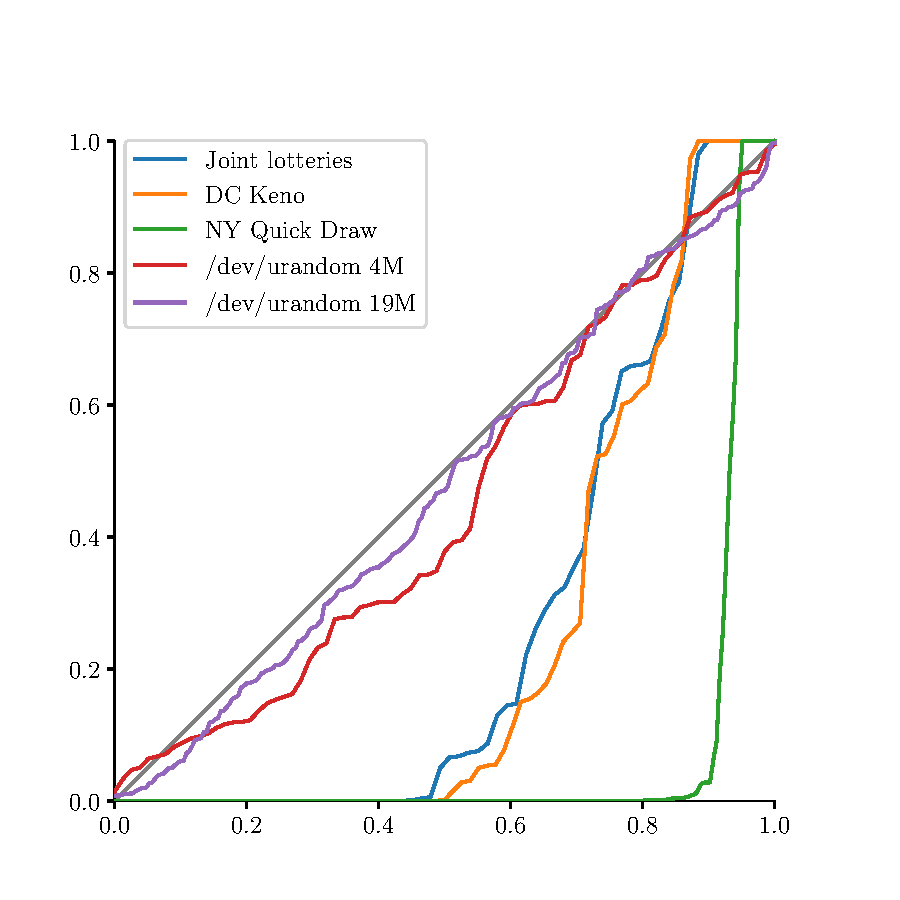
\includegraphics[width=\textwidth]{pvalue_distribution.pdf}
        \subcaption{Randomness quality as measured by Diehard. Gray line is perfect randomness.}
        \label{fig:pvalue_distribution}
    \end{subfigure}
    \hfill
    \begin{subfigure}{0.495\textwidth}
        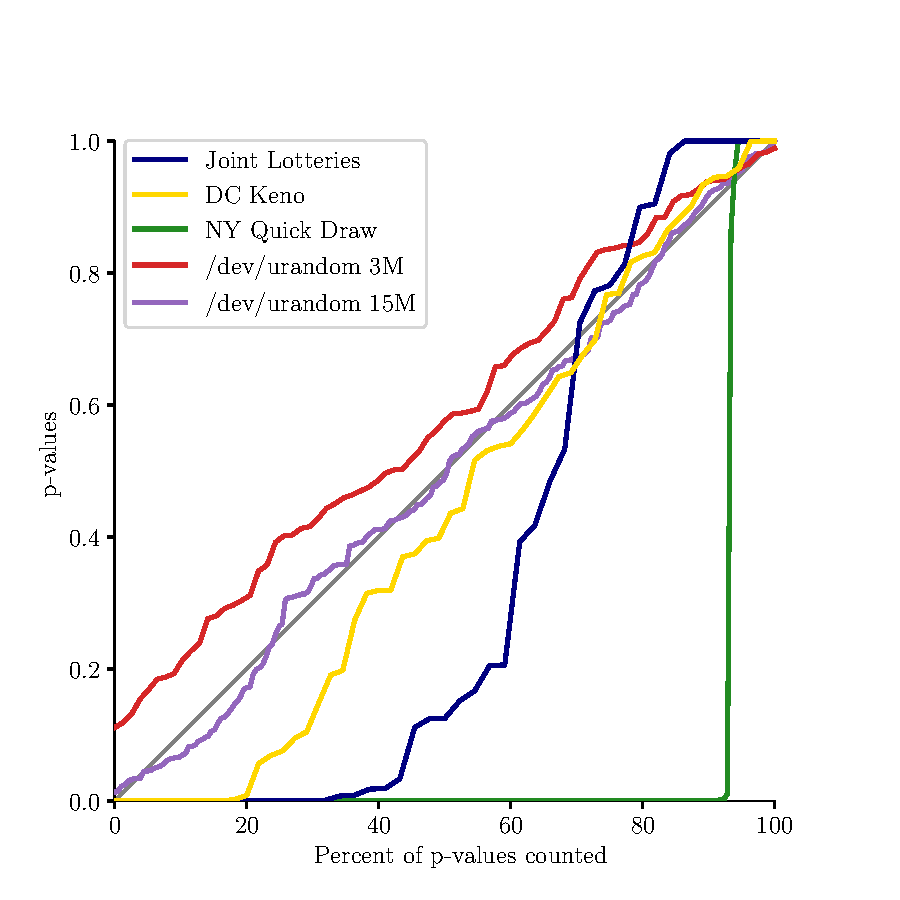
\includegraphics[width=\textwidth]{pvalue_distribution_corrected.pdf}
        \subcaption{Removed p-values from Binary Rank 6x8 test.}
        \label{fig:pvalue_corrected}
    \end{subfigure}
    \caption{p-value distribution}
\end{figure}

We immediately notice that the NY Quick Draw catastrophically failed to pass the Diehard tests. We believe this is caused
by the structure of NY Quick Draw csv files. Each row contains 20 winning numbers of an individual draw, all sorted in ascending
order. It is our opinion that Diehard identifies this ordering. This hypothesis is supported by the behaviour of Joint Lotteries
on the Runs test. This test performs two runs and provides two p-value in each run. The first run is provided a 50 \% of drawn
and 50 \% of ascending-order numbers, reports p-values of 0.981149 and 0.904974. The second run uses solely ascending-order
numbers and both p-values become 0.

The DC Keno dataset which is entirely created from drawn-order CSV files displays a remarkable even slope after it starts rising.
Curiously, the 25 of the 32 zero p-values for DC Keno come from the Binary Rank 6x8 test. If we disregard this test,
the resulting p-values are fairly uniformly distributed, although the dataset still struggles at some of them, corresponding to
20 \% of zero p-values. This is reasonable considering some enduring faults of the dataset (lottery drawn without replacement).

The Joint Lotteries mixed dataset achieves somewhat worse performance in comparison with the DC Keno dataset. We interpret this
evidence for the importance of using drawn-order input files as later runs of the same test visible degrade in performance
since they work with ascending-order numbers.

\subsection{Discussion}

There is a great number of pitfalls to take into account. Some of them have already been addressed, such as data size,
drawn/ascending order or lottery being drawn without replacement and thus not providing a truly uniformed distribution.

Furthermore, even the Diehard battery of tests possesses flaws of its own. Its critique can be found
at~\cite{dieharder, critique}. For instance, Linear Feedback Shift Registers (a type of pseudorandom number
generator) passes the Diehard battery of tests~\cite{LFSR}, despite being predictable and cryptographically weak.
